\section{Casi d'uso}
\subsection{Tipologia di utenti}
\subsection{Notazione Use Case}
\subsection{UC 1: Registrazione}
	\begin{figure}[htbp]
		\centering
		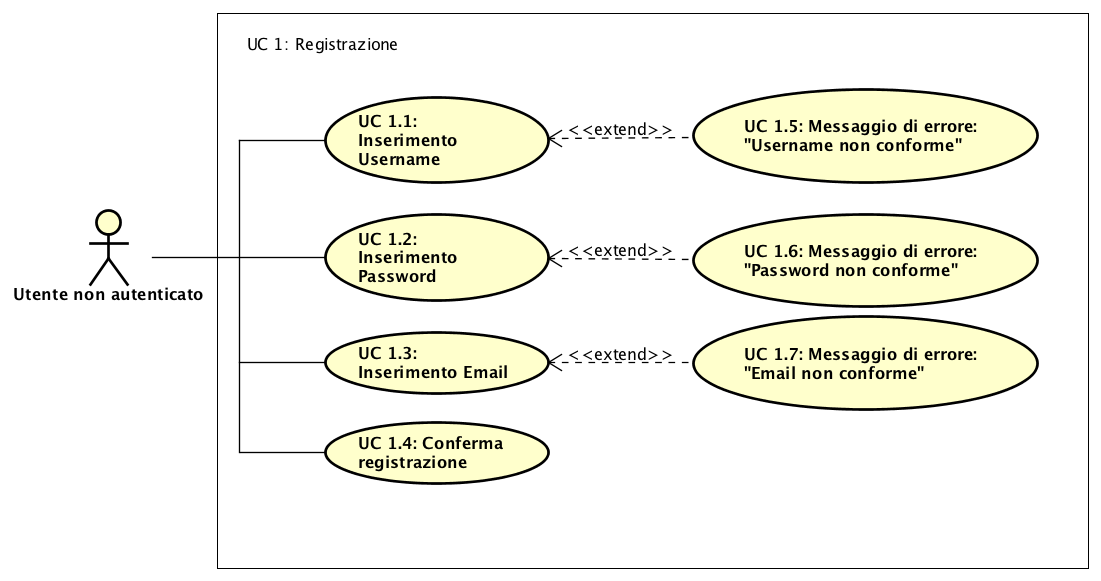
\includegraphics[scale=0.5]{../../Casi D'uso/UC1.png}
		\caption{Scelta della modalità di registrazione}
	\end{figure}
	\begin{itemize}
		\item \textbf{Attori coinvolti:}
		\item \textbf{Scopo e descrizione:} L'utente non autenticato ha selezionato l'opzione di registrazione. Tale utente deve ora decidere la modalità attraverso la quale desidera effettuare la registrazione: Standard oppure Social Network. Ad operazione avvenuta, il sistema comunicherà l'effettiva creazione dell'account indipendentemente dalla modalità scelta. \\
		\item \textbf{Precondizione:} Alla richiesta di registrazione da parte dell'utente non autenticato, il sistema fornisce le varie opzioni di registrazione. \\
		\item \textbf{Postcondizione:} Terminata l'operazione di registrazione da parte dell'utente, indipendentemente dalla modalità scelta, il sistema elabora le informazioni e restituisce, in caso affermativo, un messaggio di conferma dell'avvenuta registrazione. In caso negativo il sistema restituisce un messaggio di mancata registrazione e chiede di ripetere l'operazione. \\
	\end{itemize}
\subsection{UC 2: Autenticazione}
	\begin{figure}[h]
		\centering
		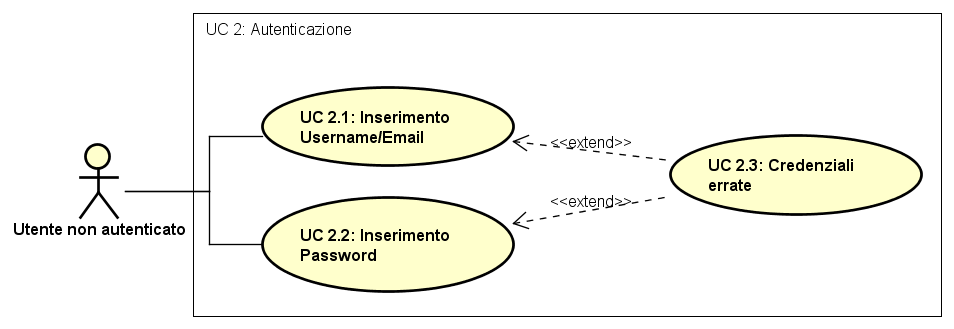
\includegraphics[scale=0.6]{../../Casi D'uso/UC2.png}
		\caption{Scelta della modalità di autenticazione}
	\end{figure}
	\begin{itemize}
		\item \textbf{Attori coinvolti:}
		\item \textbf{Scopo e descrizione:} L'utente non autenticato ha selezionato l'opzione di autenticazione. Tale utente deve ora decidere la modalità attraverso la quale desidera effettuare la registrazione: Standard oppure Social Network. \\
		\item \textbf{Precondizione:} L'utente deve aver eseguito la registrazione e quindi possedere le credenziali di accesso. Il sistema mette quindi a disposizione l'interfaccia di autenticazione. \\
		\item \textbf{Postcondizione:} Terminata l'operazione di autenticazione da parte dell'utente, indipendentemente dalla modalità scelta, il sistema elabora le informazioni e , in caso affermativo, permette di usufruire delle funzionalità specifiche di cui dispone. In caso negativo il sistema restituisce un messaggio di mancata autenticazione e chiede di ripetere l'operazione. \\
	\end{itemize}
\subsection{UC 3: Visualizzazione messaggio di errore}